
\subsection{Rhombencephalon: Metencephalon}
\label{subsec:Metencephalon} \index{Metencephalon}
%%%%%%%%%%%%%%%%%%%%%%%%%%%%%%%%%%%%%%%%%%%%%%%%%%%%%%%%%%%
%%%%%%%%%%%%%%%%%%%%%%%%%%%%%%%%%%%%%%%%%%%%%%%%%%%%%%%%%%%

Das Metencephalon oder auch Hinterhirn ist Teil des Rhombencephalons (Rautenhirn). In seiner Struktur ähnelt es dem Myelencephalon und Rückenmark. Zwischen Pons und Cerebellum, die beide im Metencephalon lokalisiert sind, verläuft der vierte Ventrikel.


\subsubsection{Pons}
\label{subsubsec:Pons} \index{Pons}
%%%%%%%%%%%%%%%%%%%%%%%%%%%%%%%%%%%%%%%%%%%%%%%%%%%%%%%%%%%

Der Pons oder das Brückenhirn beschreibt jenen Teil des Metencephalons, der direkt zwischen Mes- und Myelencephalon und inferior des Cerebellums liegt. Der Pons bildet einen von Außen gut sichtbaren, dicken Wulst, der aus vielen Fasern, aber auch aus grauer Substanz besteht. Im inferioren, bzw. ventralen Bereich, der sogenannten \textbf{Brückenhaube}, liegt das Tegmentum\index{Tegmentum! pontine} in dem einige Hirnnervenkerne lokalisiert sind. Dazu gehören der Nucleus des N. abducens und des N. facialis. Auch die Nuclei des Trapezkörpers und des medialen Lemniscus sind im Pons lokalisiert.

\begin{figure}[H]
    \centering
    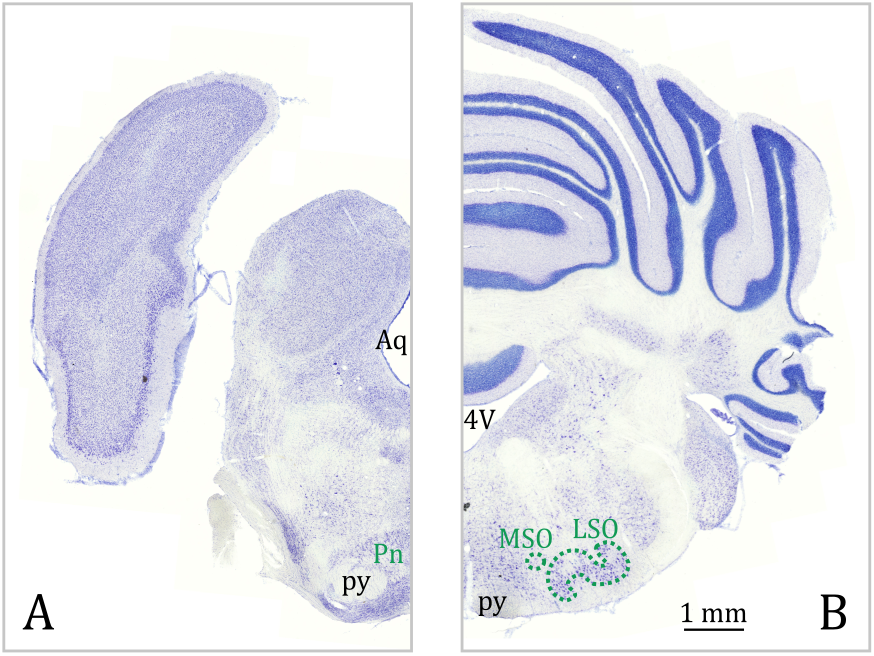
\includegraphics[width=0.7\textwidth]{pictures/Bilder_Jule/Ratte/pons.png}
    \caption[Pons Ratte]{\textbf{Pons Ratte.} Dargestellt sind ein rostraler (A:~N12-2) und caudaler (B:~N08-2) Querschnitt durch den Pons. Dabei ist rostral über dem Pons noch das Mesencephalon zu sehen, in dem sich das Aquädukt (Aq) befindet. Über dem Mesencephalon sind Teile des Cortex sichtbar. In diesem Bereich des Pons befinden sich die Nuclei pontis (Pn). Im caudalen Querschnitt ist am oberen Ende das Cerebellum sichtbar. Auch der vierte Ventrikel (4V) ist zu sehen, sowie die mediale (MSO) und laterale obere Olive (LSO). Die Pyramidenbahn (py) liegt im ventralen Bereich des Pons und erstreckt sich über dessen gesamte Länge.}
    \label{fig:pons_ratte}
\end{figure}{}

\noindent Der superiore Bereich wird auch \textbf{Brückenbasis} genannt. Sie beinhaltet die \textbf{Pyramidenbahn} und den \textbf{oberen Olivenkomplex}\index{Olive! obere Olive} (\textit{Nucleus olivaris superior}), der eine wichtige Station der Hörbahn darstellt. Ebenfalls im Pons liegen die \textbf{Nuclei pontis}\index{Nuclei! pontis}, auch Brückenkerne genannt. Diese Nuclei sind von den Fasermassen, die ihnen entspringen, bzw. zu ihnen führen, umgeben. Die meisten Afferenzen erhalten sie über den Tractus corticopontinus\index{Tractus! corticopontinus}. Dieser Trakt führt Fasern aus diversen Großhirnbereichen. Dabei erhalten die Nuclei unter anderem Informationen über Bewegungsentwürfe, die im prämotorischen Cortex ausgearbeitet werden. Nach dem die Fasern innerhalb des Pons auf die contralaterale Seite kreuzen, enden die Efferenzen in der contralateralen Kleinhirnhemisphäre. So können die Nuclei pontis die erhaltenen Informationen zur weiteren Feinabstimmung an das Kleinhirn weiterleiten. Die Nuclei pontis spielen somit eine entscheidende Rolle  bei der Verschaltung von Informationen aus dem Großhirn zum Kleinhirn \textsuperscript{\cite[Kap.~5]{trepel2011neuroanatomie}}.

\subsubsection{Cerebellum}
\label{subsubsec:Cerebellum} \index{Cerebellum! allgemein}
%%%%%%%%%%%%%%%%%%%%%%%%%%%%%%%%%%%%%%%%%%%%%%%%%%%%%%%%%%%

Das Cerebellum oder Kleinhirn ist dorsal oder superior im Metencephalon über dem Hirnstamm gelegen. Somit bedeckt es dorsal den vierten Ventrikel. Es ist durch drei Kleinhirnstiele, die \textit{Pedunculi cerebellaris}\index{Kleinhirnpedunkel}, mit dem Hirnstamm verbunden. Über diese Stiele verlaufen sowohl die Afferenzen als auch die Efferenzen des Cerebellums. Zudem ziehen zwei Kleinhirnsegel (\textit{Velum})\index{Velum} zum Mesencephalon und der Medulla. Diese Veli bestehen aus weißer Substanz und bilden das Dach des vierten Ventrikels. Bei lissencephalen\index{lissencephal} Spezies weist das Cerebellum, ähnlich wie die Großhirnrinde, viele Faltungen auf. Im direkten Vergleich sind die Falten des Cerebellums deutlich kleiner und zahlreicher. Sie verlaufen horizontal und werden auch als Blätter (\textit{Foliae}) bezeichnet \textsuperscript{\cite[Kap.~7]{trepel2011neuroanatomie}}. Eine weitere Ähnlichkeit zum Cortex besteht in der Schichtung des Cerebellums. Wie Teile der  Großhirnrinde ist auch das Kleinhirn aus drei Zellschichten aufgebaut. Die äußerste Schicht ist die \textbf{Molekularschicht} unter der die \textbf{Purkinje-Zellschicht} liegt. Die innerste Schicht ist die \textbf{Körnerzellschicht} (Abb.~\ref{fig:cerebellum_ratte}) \textsuperscript{\cite[Kap.~14]{penzlin2005tierphys}}.

\begin{figure}[H]
    \centering
    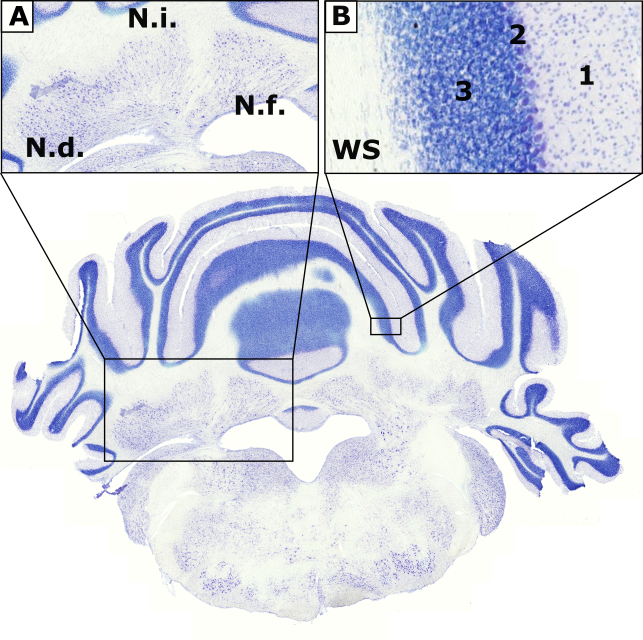
\includegraphics[width=0.8\textwidth]{pictures/Bilder_Jule/Ratte/cerebellum.png}
    \caption[Kleinhirnkerne und Schichtung des Cerebellum]{\textbf{Schichtung Cerebellum.} Ausschnitt des Cerebellums, unter dem sich der Pons befindet (N07-1). Zwischen Pons und Cerebellum ist der vierte Ventrikel sichtbar. \textbf{A} zeigt ein Ausschnitt, auf dem die drei Kleinhirnkerne, (Nucleus dentatus, N.d., der Nucleus interpositus, N.i., und der Nucleus fastigii, N.f.) zu sehen sind. \textbf{B}: Gekennzeichnet sind die weiße Substanz (WS), sowie die drei Schichten der grauen Substanz. Die äußerste Schicht ist die Molekularschicht (\textbf{1}). Weiter innen liegen die Purkinje-Zellschicht (\textbf{2}) und die Körnerzellschicht (\textbf{3}).}
    \label{fig:cerebellum_ratte}
\end{figure}

\noindent Aufgrund der verschiedenen afferenten Faserverbindungen lässt sich das Cerebellum in drei Gebiete gliedern: Das \textbf{Vestibulocerebellum}\index{Cerebellum! Vestibulocerebellum} erhält Afferenzen aus aus dem Vestibularapparat des Innenohrs, das \textbf{Spinocerebellum}\index{Cerebellum! Spinocerebellum} aus dem Rückenmark und das \textbf{Corticocerebellum}\index{Cerebellum! Corticocerebellum} aus den Nuclei pontis. Des Weiteren liegen im Cerebellum die \textbf{Kleinhirnkerne}, zu denen der Nucleus dentatus, der Nucleus interpositus und der Nucleus fastigii gehören. Das Cerebellum spielt eine wichtige Rolle für die Koordination von Haltung und Bewegung und gilt generell als motorisches Koordinationszentrum (Kap.~\ref{sub:kleinhirn}) \textsuperscript{\cite[Kap.~7]{trepel2011neuroanatomie}}.
